\حصہ{خط بندی اور تفرقات}
بعض اوقات پیچیدہ تفاعل کو سادہ تخمینی تفاعل سے  ظاہر کرتے ہوئے مخصوص موقعوں پر قابل قبول نتائج حاصل کرنا ممکن ہوتا ہے۔ ان سادہ تفاعل کے ساتھ کام کرنا زیادہ آسان ثابت ہوتا ہے۔ اس حصہ میں مماس پر مبنی \اصطلاح{خط بندی}\حاشیہب{linearizations} پر غور کیا گیا ہے۔

ہم نئے متغیرات \عددی{\dif x} اور \عددی{\dif y} متعارف کرتے ہیں جو \عددی{\tfrac{\dif y}{\dif x}} کو نئی معنی دیں گے۔  ہم تجرباتی پیمائش میں خلل اور حساسیت  کو \عددی{\dif y} سے ظاہر کریں گے۔

\جزوحصہء{خطی تخمین}
آپ شکل \حوالہ{شکل_استعمال_منحنی_اور_مماس} میں دیکھ سکتے ہیں کہ منحنی \عددی{y=f(x)} کا مماس نقطہ مماس کے نزدیک منحنی کے قریب رہتا ہے۔نقطہ مماس کے دونوں اطراف چھوٹے وقفہ پر مماس کی \عددی{y} قیمت کو  منحنی کی \عددی{y} تخمینی قیمت تصور کیا جا سکتا ہے۔
\begin{figure}
\centering
\begin{subfigure}{0.5\textwidth}
\centering
\begin{tikzpicture}[font=\small]
\begin{axis}[small,axis lines=middle,xlabel={$x$},ylabel={$y$}]
\addplot[domain=-1:2]{x^2}node[pos=0.9,left]{$y=x^2$};
\addplot[domain=0.2:2]{2*x-1}node[pos=0.7,sloped, below]{$y=2x-1$};
\draw(axis cs:1,1)node[circ]{}node[left]{$(1,1)$};
\end{axis}
\end{tikzpicture}
\caption{منحنی اور اس کا نقطہ $(1,1)$ پر مماس}
\end{subfigure}%
\begin{subfigure}{0.5\textwidth}
\centering
\begin{tikzpicture}[font=\small]
\begin{axis}[small,axis lines=middle,xlabel={$x$},ylabel={$y$}]
\addplot[domain=0.5:1.5]{x^2}node[pos=0.9,left]{$y=x^2$};
\addplot[domain=0.5:1.5]{2*x-1}node[pos=0.7,sloped, below]{$y=2x-1$};
\draw(axis cs:1,1)node[circ]{}node[left]{$(1,1)$};
\end{axis}
\end{tikzpicture}
\caption{نقطہ $(1,1)$ کے نزدیک منحنی اور مماس قریب قریب ہیں}
\end{subfigure}
\begin{subfigure}{0.5\textwidth}
\centering
\begin{tikzpicture}[font=\small]
\begin{axis}[small,axis lines=middle,xlabel={$x$},ylabel={$y$}]
\addplot[domain=0.9:1.11]{x^2}node[pos=0.9,left]{$y=x^2$};
\addplot[domain=0.9:1.11]{2*x-1}node[pos=0.7,sloped, below]{$y=2x-1$};
\draw(axis cs:1,1)node[circ]{}node[left]{$(1,1)$};
\end{axis}
\end{tikzpicture}
\caption{دکھائے گئے وقفہ پر مماس اور منحنی بہت قریب ہیں}
\end{subfigure}%
\begin{subfigure}{0.5\textwidth}
\centering
\begin{tikzpicture}[font=\small]
\begin{axis}[small,axis lines=middle,xlabel={$x$},ylabel={$y$},xtick={0.998,1.002,1},xticklabels={$0.998$,$1.002$,$1$},ytick={0.998,1,1.002},yticklabels={$0.998$,$1$,$1.002$},xmin=0.997]
\addplot[domain=0.998:1.002]{x^2}node[pos=0.9,left]{$y=x^2$};
\addplot[domain=0.998:1.002]{2*x-1}node[pos=0.7,sloped, below]{$y=2x-1$};
\draw(axis cs:1,1)node[circ]{}node[left]{$(1,1)$};
\end{axis}
\end{tikzpicture}
\caption{دکھائے گئے وقفے پر منحنی اور مماس میں فرق کرنا مشکل ہے}
\end{subfigure}
\caption{قابل تفرق منحنی کو نقطہ مماس کے قریب  تخمینی طور پر اس  نقطے کے  مماس سے ظاہر کیا جا سکتا ہے}
\label{شکل_استعمال_منحنی_اور_مماس}
\end{figure}

شکل \حوالہ{شکل_استعمال_منحنی_کا_مماس} کی علامتیت استعمال کرتے ہوئے، نقطہ \عددی{(a,f(a))} سے گزرتے ہوئے مماس کی نقطہ-ڈھلوان مساوات
\begin{align*}
y=f(a)+f'(a)(x-a)
\end{align*}
ہے۔یوں مماس درج ذیل تفاعل
\begin{align*}
L(x)=f(a)+f'(a)(x-a)
\end{align*}
کی ترسیم ہے۔ جب تک یہ خط منحنی کے نزدیک رہے اس کو \عددی{f(x)} کی تخمین تصور کیا جا سکتا ہے۔
\begin{figure}
\centering
\begin{tikzpicture}[font=\small]
\begin{axis}[small,axis lines=middle,xlabel={$x$},ylabel={$y$},xtick={\empty},ytick={\empty},xmin=0,ymin=-0.25]
\addplot[domain=0.5:1.5]{x^2}node[pos=0.9,left]{$y=f(x)$};
\addplot[domain=0.6:1.5]{2*x-1}node[pos=0.7,sloped, below]{$f'(a)$ ڈھلوان};
\draw(axis cs:1,1)node[circ]{}node[left]{$(a,f(a))$};
\draw[dashed](axis cs:1,1)--(axis cs:1,0)node[below]{$a$};
\end{axis}
\end{tikzpicture}
\caption{نقطہ $a$ پر تفاعل $f(x)$ کا مماس $y=f(a)+f'(a)(x-a)$ ہو گا}
\label{شکل_استعمال_منحنی_کا_مماس}
\end{figure}

\ابتدا{تعریف}\\
اگر \عددی{x=a} پر \عددی{f} قابل تفرق ہو تب تخمینی تفاعل
\begin{align}\label{مساوات_استعمال_خطی_تخمین}
L(x)=f(a)+f'(a)(x-a)
\end{align}
نقطہ \عددی{a} پر \عددی{f} کی \اصطلاح{خط بندی}\فرہنگ{خط بندی}\حاشیہب{linearization}\فرہنگ{linearization} ہو گی۔  \عددی{f} کی درج ذیل تخمین \عددی{L}
\begin{align*}
f(x)\approx L(x)
\end{align*}
نقطہ \عددی{a} پر تفاعل \عددی{f}کی \اصطلاح{معیاری خطی تخمین}\فرہنگ{خطی!معیاری تخمین}\حاشیہب{standard linear approximation}\فرہنگ{linear!standard approximation} ہے۔ نقطہ \عددی{x=a} اس تخمین کا \اصطلاح{وسط}\فرہنگ{وسط}\حاشیہب{center}\فرہنگ{center} ہے۔
\انتہا{تعریف}
%=========================

\ابتدا{مثال}\شناخت{مثال_استعمال_تخمینی_صورت_الف}
\عددی{x=0} پر \عددی{f(x)=\sqrt{1+x}} کی خط بندی تلاش کریں۔\\
حل:\quad
ہم \عددی{a=0} پر مساوات \حوالہ{مساوات_استعمال_خطی_تخمین} کی درکار صورت حاصل کرتے ہیں جہاں
\begin{align*}
f'(x)=\frac{1}{2}(1+x)^{-\tfrac{1}{2}}
\end{align*}
لیتے ہوئے \عددی{f(0)=1} اور \عددی{f'(0)=\tfrac{1}{2}} ہوں گے لہٰذا
\begin{align*}
L(x)=f(a)+f'(a)(x-a)=1+\frac{1}{2}(x-0)=1+\frac{x}{2}
\end{align*}
ہو گا۔ شکل \حوالہ{شکل_مثال_استعمال_تخمینی_صورت_الف}-الف میں منحنی اور مماس دکھائے گئے ہیں۔ شکل-ا میں مماسی نقطہ کو ڈبہ میں دکھایا گیا ہے۔اس ڈبے کو شکل-ب میں بڑا کر کے دکھایا گیا ہے۔
\انتہا{مثال}
%==========================
\begin{figure}
\centering
\begin{subfigure}{0.45\textwidth}
\centering
\begin{tikzpicture}[font=\small]
\begin{axis}[clip=false,small,axis lines=middle,xlabel={$x$},ylabel={$y$},xlabel style={at={(current axis.right of origin)},anchor=west},ylabel style={at={(current axis.above origin)},anchor=south},xmin=-1.25]
\addplot[domain=-1:-0.5]{sqrt(1+x)};
\addplot[domain=-0.5:5.2]{sqrt(1+x)}node[pos=0.5,below right]{$y=\sqrt{1+x}$};
\addplot[domain=-1:2]{1+x/2}node[pos=0.75,sloped,above]{$y=1+\tfrac{x}{2}$};
\addplot[domain=1.5:5]{5/4+x/4}node[pos=0.8,sloped,above]{$y=\tfrac{5}{4}+\tfrac{x}{4}$};
\draw(axis cs:0,1)node[circ]{};
\draw(axis cs:3,2)node[circ]{};
\draw(axis cs:-0.2,0.9) rectangle (axis cs:0.2,1.1);
\end{axis}
\end{tikzpicture}
\caption{}
\end{subfigure}\hfill
\begin{subfigure}{0.45\textwidth}
\centering
\begin{tikzpicture}[font=\small]
\begin{axis}[clip=false,small,axis lines=middle,xlabel={$x$},ylabel={$y$},xlabel style={at={(current axis.right of origin)},anchor=west},ylabel style={at={(current axis.above origin)},anchor=south},xmin=-0.11,xmax=0.25,ymin=0.85,ymax=1.15,xtick={-0.1,0.1,0.2},ytick={0.9,1.0,1.1}]
\addplot[domain=-0.1:0.2]{sqrt(1+x)}node[pos=0.8,pin=120:{$y=\sqrt{1+x}$}]{};
\addplot[domain=-0.1:0.2]{1+x/2}node[pos=0.75,pin=-45:{$y=1+\tfrac{x}{2}$}]{};
\end{axis}
\end{tikzpicture}
\caption{}
\end{subfigure}
\caption{نقطہ $x=0$ پر $y=\sqrt{1+x}$ اور اس کی خط بندی۔}
\label{شکل_مثال_استعمال_تخمینی_صورت_الف}
\end{figure}


تخمین \عددی{\sqrt{1+x}\approx 1+\tfrac{x}{2}} (شکل \حوالہ{شکل_مثال_استعمال_تخمینی_صورت_الف}-ب) سے درج ذیل قیمتیں حاصل ہوتی ہیں۔
\begin{align*}
\sqrt{1.2}&\approx 1+\frac{0.2}{2}=1.10&& \text{\RL{$2$ اعشاریہ درست}}\\
\sqrt{1.05}&\approx 1+\frac{0.05}{2}=1.025&& \text{\RL{$3$ اعشاریہ درست}}\\
\sqrt{1.005}&\approx 1+\frac{0.005}{2}=1.00250&& \text{\RL{$5$ اعشاریہ درست}}\\
\end{align*}

وسط سے دور خط بندی میں خلل نا قابل نظر انداز ہو گا۔یوں \عددی{\sqrt{1+x}=1+\tfrac{x}{2}} کو \عددی{x=3} کے نزدیک استعمال نہیں کیا جا سکتا ہے۔ آپ کو \عددی{x=3} پر نئی خط بندی حاصل کرنی ہو گی۔

\ابتدا{مثال}
\عددی{x=3} پر تفاعل \عددی{f(x)=\sqrt{1+x}} کی خط بندی حاصل کریں۔ \\
حل:\quad
ہم \عددی{a=3} پر مساوات \حوالہ{مساوات_استعمال_خطی_تخمین} کی درکار صورت حاصل کرتے ہیں جہاں
\begin{align*}
f(3)=2,\quad f'(3)=\left.\frac{1}{2}(1+x)^{-\tfrac{1}{2}}\right|_{x=3}=\frac{1}{4}
\end{align*}
ہے لہٰذا
\begin{align*}
L(x)=2+\frac{1}{4}(x-3)=\frac{5}{4}+\frac{x}{4}
\end{align*}
ہو گا (شکل \حوالہ{شکل_مثال_استعمال_تخمینی_صورت_الف}-ا)۔ اس خط بندی سے \عددی{x=3.2} پر 
\begin{align*}
\sqrt{1+x}=\sqrt{1+3.2}\approx \frac{5}{4}+\frac{3.2}{4}=1.250+0.800=2.050
\end{align*}
حاصل ہوتا ہے جو بالکل درست جواب \عددی{\sqrt{4.2}\approx 2.04939} سے \عددی{\num{0.00061}} ہٹ کر ہے۔

اگر ہم مثال \حوالہ{مثال_استعمال_تخمینی_صورت_الف} میں حاصل خط بندی استعمال کریں تب 
\begin{align*}
\sqrt{+x}=\sqrt{1+3.2}\approx 1+\frac{3.2}{2}=1+1.6=2.6
\end{align*}
حاصل ہو گا جس میں \عددی{\SI{25}{\percent}} خلل پایا جاتا ہے۔
\انتہا{مثال}
%================
\ابتدا{مثال}
جذروں اور طاقتوں کے لئے اہم ترین خط بندی درج ذیل ہے۔
\begin{align}\label{مساوات_استعمال_طاقت_خطی_تخمین}
(1+x)^k&\approx 1+kx&&\text{\RL{$k$ کوئی عدد ہے؛ $x\approx 0$}}
\end{align}
\عددی{x=0} کے نزدیک یہ قابل قبول نتائج دیتا ہے اور یہ وسیع طور استعمال ہوتا ہے۔
\انتہا{مثال}
%===========================

مساوات \حوالہ{مساوات_استعمال_طاقت_خطی_تخمین} سے درج ذیل کلیات اخذ کیے جا سکتے ہیں جن کا وسط \عددی{x=0} ہے۔
\begin{align*}
\sqrt{1+x}&=(1+x)^{\tfrac{1}{2}}\approx 1+\frac{x}{2}&& k=\frac{1}{2}\\
\frac{1}{1-x}&=(1-x)^{-1}\approx 1+(-1)(-x)=1+x&&k=-1\\
\sqrt[3]{1+5x^4}&=(1+5x^4)^{\tfrac{1}{3}}=1+\frac{1}{3}(5x^4)=1+\frac{5}{3}x^4&&k=\frac{1}{3}\\
\frac{1}{\sqrt{1-x^2}}&=(1-x^2)^{-\tfrac{1}{2}}\approx 1+(-\tfrac{1}{2})(-x^2)=1+\frac{x^2}{2}&&k=-\frac{1}{2}
\end{align*}
دیگر اہم خط بندی درج ذیل ہیں (اس حصہ کے آخر میں دیے سوالات میں  آپ انہیں اخذ کریں گے) جن کا وسط \عددی{x=0} ہے۔
\begin{align*}
\sin x&\approx x\\
\cos x&\approx 1\\
\tan x&\approx x
\end{align*}
\ابتدا{مثال}\شناخت{مثال_استعمال_خطی_تخمین_کوسائن}
\عددی{x=\tfrac{\pi}{2}} پر \عددی{f(x)=\cos x} کی خط بندی حاصل کریں۔\\
حل:\quad
درج ذیل
\begin{align*}
f(\tfrac{\pi}{2})=\cos(\tfrac{\pi}{2})=0,\quad f'(\tfrac{\pi}{2})=-\sin(\tfrac{\pi}{2})=-1
\end{align*}
لیتے ہوئے خط بندی درج ذیل ہو گی (شکل \حوالہ{شکل_مثال_استعمال_خطی_تخمین_کوسائن})۔
\begin{align*}
L(x)=f(a)+f'(a)(x-a)=0+(-1)(x-\tfrac{\pi}{2})=-x+\tfrac{\pi}{2}
\end{align*}
\انتہا{مثال}
%=============================
\begin{figure}
\centering
\begin{tikzpicture}
\pgfmathsetmacro{\a}{3/2*pi}
\pgfmathsetmacro{\b}{pi/2}
\begin{axis}[clip=false,small,axis lines=middle,xlabel={$x$},ylabel={$y$},xlabel style={at={(current axis.right of origin)},anchor=west},ylabel style={at={(current axis.above origin)},anchor=south},ymax=1.5,xmax=5.2,xtick={\b},xticklabels={$\tfrac{\pi}{2}$},ytick={\empty}]
\addplot[domain=-\a/6:\a,smooth]{cos(deg(x))}node[pos=0.75,below right]{$y=\cos x$};
\addplot[domain=0.3:3]{-x+pi/2}node[pos=0.1, above right]{$y=-x+\tfrac{\pi}{2}$};
\end{axis}
\end{tikzpicture}
\caption{کوسائن اور نقطہ $x=\tfrac{\pi}{2}$ پر اس کی خط بندی۔}
\label{شکل_مثال_استعمال_خطی_تخمین_کوسائن}
\end{figure}

\جزوحصہء{تفرقات}
\ابتدا{تعریف}\\
فرض کریں \عددی{y=f(x)} قابل تفرق تفاعل ہے۔ \موٹا{تفرق} \عددی{\dif x} غیر تابع متغیر ہے۔ \موٹا{تفرق} \عددی{\dif y} درج ذیل ہے۔
\begin{align*}
\dif y=f'(x)\dif x
\end{align*}
\انتہا{تعریف}
%===================

عموماً تفرق \عددی{\dif x} غیر تابع متغیر میں تبدیلی \عددی{\Delta x}ہو گی۔ البتہ تعریف ہیں ہم \عددی{\dif x}پر یہ شرط لاگو نہیں کرتے ہیں۔ تفرق \عددی{\dif y} ہر صورت تابع ہو گا اور اس کی قیمت \عددی{x} اور \عددی{\dif x} پر منحصر ہو گی۔

\ابتدا{مثال}
\عددی{y=x^5+37x} اور \عددی{y=\sin 3x} کے لئے \عددی{\dif y} تلاش کریں۔\\
حل:
\begin{align*}
\dif y=(5x^4+37)\dif y,\quad \dif y=(3\cos 3x)\dif x
\end{align*}
\انتہا{مثال}
%====================
اگر \عددی{\dif x\ne 0} ہو تب ہم مساوات \عددی{\dif y=f'(x)\dif x} کے دونوں اطراف کو \عددی{\dif x} سے تقسیم کر کے جانی پہچانی مساوات
\begin{align*}
\frac{\dif y}{\dif x}=f'(x)
\end{align*}
حاصل کرتے ہیں۔ یہ مساوات کہتی ہے کہ \عددی{\dif x\ne 0} کی صورت میں \عددی{f'(x)} تفرقات کا حاصل تقسیم ہو گا۔

بعض اوقات ہم \عددی{\dif f'(x)\dif x} کی بجائے 
\begin{align*}
\dif f=f'(x)\dif x
\end{align*}
لکھتے ہیں اور \عددی{\dif f} کو \عددی{f} کا \اصطلاح{تفرق} کہتے ہیں۔ مثال کے طور پر \عددی{f(x)=3x^2-6} کی صورت میں
\begin{align*}
\dif f=\dif (3x^2-6)=6x\dif x
\end{align*}
ہو گا۔

تفرق کے ہر کلیہ مثلاً
\begin{align*}
\frac{\dif(u+v)}{\dif x}=\frac{\dif u}{\dif x}+\frac{\dif v}{\dif x}
\end{align*}
 کے دونوں اطراف کو \عددی{\dif x} سے ضرب دے کر مطابقتی تفرقی روپ
\begin{align*}
\dif (u+v)=\dif u+\dif v
\end{align*}
حاصل ہو گی۔ چند تفرقی کلیات پیش کرتے ہیں۔
\begin{align*}
\begin{array}{lll}
\dif c=0,&\dif (cu)=c\dif u,&\dif (u+v)=\dif u+\dif v,\\
\dif(uv)=u\dif v+v\dif u,&\dif(\tfrac{u}{v})=\frac{v\dif u-u\dif v}{v^2},&\dif (u^n)=nu^{n-1}\dif u,\\
\dif(\sin u)=\cos u\dif u,&\dif (\cos u)=-\sin u \dif u,&\dif (\tan u)=\sec^2u\dif u,\\
\dif (\cot u)=-\csc^2u\dif u,&\dif(\sec u)=\sec u\tan u\dif u,&\dif(\csc u)=-\csc u\cot u\dif u
\end{array}
\end{align*}

\ابتدا{مثال}
\begin{align*}
\dif(\tan 2x)&=\sec^2(2x)\dif (2x)=2\sec^2 2x\dif x\\
\dif(\tfrac{x}{x+1})&=\frac{(x+1)\dif x-x\dif(x+1)}{(x+1)^2}=\frac{x\dif x+\dif x-x\dif x}{(x+1)^2}=\frac{\dif x}{(x+1)^2}
\end{align*}
\انتہا{مثال}
%=====================
\جزوحصہء{تفرقات کی مدد سے تبدیلی کی اندازاً قیمت}
فرض کریں نقطہ \عددی{x_0} پر قابل تفرق تفاعل \عددی{f(x)} کی قیمت ہم جانتے ہیں۔ہم جاننا چاہتے ہیں کہ کسی نزدیک نقطہ \عددی{x_0+\dif x} پر جانے سے تفاعل کی قیمت میں تبدیلی کتنی ہو گی۔ اگر \عددی{\dif x} نہایت کم ہو تب \عددی{f} اور \عددی{x_0} پر اس کی خط بندی \عددی{L} ایک دوسرے کے برابر  تبدیل ہوں گے۔ چونکہ \عددی{L} کا حساب زیادہ آسان ہے لہٰذا اس کی مدد لینا سود مند ثابت ہو گا۔

شکل \حوالہ{شکل_استعمال_تفرقی_خطی} میں دیے علامتوں کو استعمال کرتے ہوئے \عددی{f} میں تبدیلی لکھتے ہیں۔
\begin{align*}
\Delta f=f(x_0+\dif x)-f(x_0)
\end{align*}
\عددی{L} میں مطابقتی تبدیلی درج ذیل ہو گی۔
\begin{align*}
\Delta L&=L(x_0+\dif x)-L(x_0)\\
&=\underbrace{f(x_0)+f'(x_0)[(x_0+\dif x)-x_0]}_{L(x_0+\dif x)}-\underbrace{f(x_0)}_{L(x_0)=f(x_0)}\\
&=f'(x_0)\dif x
\end{align*}

تفرق \عددی{\dif f=f'(x)\dif x} کا جیومیٹریائی مطلب پر غور کریں۔ جب \عددی{x=x_0} پر \عددی{\dif f} کی قیمت حاصل کی جائے تب \عددی{\dif f=\Delta L} ہو گا یعنی خط بندی میں تبدیل \عددی{\dif f} کے برابر ہو گی۔
\begin{figure}
\centering
\begin{tikzpicture}[declare function={fa(\x)=\x*\x+1; fb(\x)=2*\x;}]
\pgfmathsetmacro{\a}{1}
\pgfmathsetmacro{\b}{1.75}
\pgfmathsetmacro{\nA}{fa(\a)}
\pgfmathsetmacro{\nB}{fb(\b)}
\pgfmathsetmacro{\nC}{fa(\b)}
\begin{axis}[clip=false,small,axis lines=middle,xlabel={$x$},ylabel={$y$},xmin=0,ymin=0,xtick={1,1.75},xticklabels={$x_0$,$x_0+\dif x$},ytick={\empty},xmax=2.5]
\addplot[domain=0.5:2]{fa(x)}node[left]{$y=f(x)$};
\addplot[domain=0.5:1.87]{fb(x)}node[pos=0,below]{مماس};
\draw[dashed](axis cs:\a,\nA)node[left]{$(x_0,f(x_0))$}--(axis cs:\a,0);
\draw[dashed](axis cs:\b,\nA)--(axis cs:\b,0);
\draw(axis cs:\a,\nA)--(axis cs:\b,\nA)node[pos=0.5,below]{$\dif x$}--(axis cs:\b,\nB);
\draw[dashed](axis cs:\b,\nB)--(axis cs:\b,\nC);
\draw[stealth-stealth](axis cs:\b+0.2,\nA)--(\b+0.2,\nB)node[pos=0.4,right]{$\Delta L=f'(x_0)\dif x$};
\draw(axis cs:\b+0.1,\nA)--(axis cs:\b+1.75,\nA);
\draw(axis cs:\b+0.1,\nB)--(axis cs:\b+0.3,\nB);
\draw[](axis cs:\b+0.1,\nC)--(axis cs:\b+1.75,\nC);
\draw[stealth-stealth](axis cs:\b+1.7,\nA)--(axis cs:\b+1.7,\nC)node[pos=0.65,fill=white]{$\Delta f=f(x_0+\dif x)-f(x_0)$};
\end{axis}
\end{tikzpicture}
\caption{چھوٹے $\dif x$ کی صورت میں $f$ کی خط بندی تقریباً $f$ میں تبدیلی کے برابر ہو گی۔ }
\label{شکل_استعمال_تفرقی_خطی}
\end{figure}
\موٹا{تفرقی تبدیلی کی اندازاً قیمت}\\
فرض کریں \عددی{x=x_0} پر \عددی{f(x)} قابل تفرق ہے۔ \عددی{x} کی قیمت \عددی{x_0} سے \عددی{x_0+\dif x} کرنے سے \عددی{f} میں تبدیلی تخمیناً درج ذیل ہو گا۔
\begin{align*}
\dif f=f'(x_0)\dif x
\end{align*}

\ابتدا{مثال}
ایک دائرے کا رداس \عددی{r_0=\SI{10}{\centi\meter}} سے \عددی{\SI{10.1}{\centi\meter}} کیا جاتا ہے۔ \عددی{\dif S} کا حساب کرتے ہوئے ہوئے اس کے رقبہ \عددی{S} میں تبدیلی حاصل کریں۔ اس کا موازنہ حقیقی تبدیلی \عددی{\Delta S} کے ساتھ کریں۔\\
حل:\quad
چونکہ \عددی{S=\pi r^2} ہے لہٰذا اندازاً تبدیلی
\begin{align*}
\dif S=S'(r_0)\dif r=2\pi r_0\dif r=2\pi(10)(0.1)=2\pi\,\si{\meter\squared}
\end{align*}
ہو گی۔حقیقی تبدیل درج ذیل ہے۔
\begin{align*}
\Delta S=\pi (10.1)^2-\pi (10)^2=(102.01-100)\pi=\underbrace{2\pi}_{\dif S}+\underbrace{0.01\pi}_{\text{خلل}}
\end{align*}
\انتہا{مثال}
%===================
\جزوحصہء{مطلق، اضافی، اور فی صد تبدیلی}
\عددی{x_0} سے نزدیک نقطہ \عددی{x_0+\dif x} منتقل ہوتے ہوئے ہم \عددی{f} میں تبدیلی کو تین طریقوں سے ظاہر کر سکتے ہیں جنہیں جدول \حوالہ{جدول_استعمال_تبدیلی_اظہار} میں دکھایا گیا ہے۔
\begin{table}
\caption{تبدیلی کے اظہار کے تین طریقے}
\label{جدول_استعمال_تبدیلی_اظہار}
\centering
\begin{tabular}{lll}
&اصل &اندازاً\\
\hline
حتمی تبدیلی & $\Delta f=f(x_0+\dif x)-f(x_0)$&$\dif f=f'(x_0)\dif x$\\
اضافی تبدیلی&$\frac{\Delta f}{f(x_0)}$&$\frac{\dif f}{f(x_0)}$\\
فی صد تبدیلی&$\frac{\Delta f}{f(x_0)}\times 100$&$\frac{\dif f}{f(x_0)}\times 100$\\
\end{tabular}
\end{table}

\ابتدا{مثال}
گزشتہ مثال میں فی صف اندازاً تبدیلی درج ذیل ہے۔
\begin{align*}
\frac{\dif S}{S(r_0)}\times 100=\frac{2\pi}{100\pi}\times 100=\SI{2}{\percent}
\end{align*} 
\انتہا{مثال}
%=====================
\ابتدا{مثال}\ترچھا{زمین کا سطحی رقبہ}\\
زمین کو کرہ تصور کریں جس کا رداس \عددی{6371\mp 0.1\,\si{\kilo\meter}} ہے۔زمین کے رقبہ میں خلل کتنا ہو گا؟\\
حل:\quad
رداس \عددی{r} کے کرہ کا سطحی رقبہ \عددی{S=4\pi r^2} ہوتا ہے۔ \عددی{r} میں خلل کی بنا \عددی{S} میں خلل درج ذیل ہو گا۔
\begin{align*}
\dif S=\big(\frac{\dif S}{\dif r}\big)\dif r=8\pi r\dif r=8\pi(6371)(0.1)=\SI{16012}{\kilo\meter\squared}
\end{align*}
\انتہا{مثال}
%=========================
\ابتدا{مثال}
رداس \عددی{r} کے کرہ کا رقبہ \عددی{\SI{1}{\percent}} درست حاصل کرنے کی خاطر اس کا رداس کتنا درست ناپنا ہو گا؟\\
حل:\quad
ہم چاہتے ہیں کہ رداس میں تبدیلی اتنی کم ہو کہ درج ذیل مطمئن ہوتا ہو۔
\begin{align*}
\abs{\Delta S}\le \frac{S}{100}=\frac{4\pi r^2}{100}
\end{align*}
ہم اس عدم مساوات میں \عددی{\Delta s} کی جگہ 
\begin{align*}
\dif S=\big(\frac{\dif S}{\dif r}\big)\dif r=8\pi r\dif r
\end{align*}
پر کرتے ہیں۔یوں
\begin{align*}
\abs{8\pi r\dif r}\le \frac{4\pi r^2}{100}\quad \implies \quad \abs{\dif r}\le \frac{1}{8\pi r}\cdot \frac{4\pi r^2}{100}=\frac{1}{2}\frac{r}{100}
\end{align*}
حاصل ہوتا ہے۔یوں رداس میں خلل اصل رداس کے \عددی{\SI{0.5}{\percent}} سے کم ہونا ضروری ہے۔
\انتہا{مثال}
%=========================
\ابتدا{مثال}\شناخت{مثال_استعمال_شریانہ}\ترچھا{بند شریانوں کا کھولنا (انجیوپلاسٹی\فرہنگ{انجیوپلاسٹی}\حاشیہب{angioplasty}\فرہنگ{angioplasty})}

جزوی طور پر بند شریانوں کی رداس کو بڑا کرتے ہوئے خون کی عمومی بہاو حاصل کی جا سکتی ہے۔  \سن{1830} کے لگ بھگ فرانس کے جین پوزوئے نے درج ذیل کلیہ اخذ کیا
\begin{align*}
H=&kr^4&& \text{\RL{($k$ مستقل)}}
\end{align*}
جو مستقل دباو پر  فی اکائی وقت میں  ایک چھوٹی نالی میں حجم بہاو \عددی{H} دیتا ہے۔ اس نالی کا رداس \عددی{r} ہے۔رداس  \عددی{\SI{10}{\percent}} بڑھانے  سے بہاو پر کیا اثر ہو گا؟\\
حل:\quad
\عددی{r} اور \عددی{H} کے تفرقات کا تعلق لکھتے ہیں۔
\begin{align*}
\dif H=\frac{\dif H}{\dif r}\dif r=4kr^3\dif r
\end{align*}
یوں
\begin{align*}
\frac{\dif H}{H}=\frac{4kr^3\dif r}{kr^4}=4\frac{\dif r}{r}
\end{align*}
ہو گا یعنی \عددی{H} میں اضافی تبدیل \عددی{r} کی اضافی تبدیلی کے \عددی{4} گنا ہے۔یوں \عددی{r} میں \عددی{\SI{10}{\percent}} تبدیلی سے \عددی{H} میں \عددی{\SI{40}{\percent}} تبدیلی پیدا ہو گی۔
\انتہا{مثال}
%========================
\جزوحصہء{حساسیت}
مختلف \عددی{x} پر مساوات \عددی{\dif f=f'(x)\dif x} ہمیں  \عددی{f} کی حساسیت دیتی ہے۔\عددی{x} پر \عددی{f'} کی قیمت جتنی زیادہ ہو، کسی بھی تبدیلی \عددی{\dif x}کے لئے  \عددی{f}میں تبدیلی اتنی زیادہ ہو گی۔    

\ابتدا{مثال}\شناخت{مثال_استعمال_پل_اونچائی}
آپ ایک پل کی اونچائی ناپنے کی خاطر ایک پتھر کو پانی میں گرا کر چھینٹوں کی آواز آنے تک وقت ناپتے ہیں۔ آپ \عددی{s=4.9t^2} استعمال کرتے ہیں۔ \عددی{0.1} سیکنڈ خلل کے لحاظ سے آپ کے جواب کی حساسیت کیا ہو گی؟\\
حل:\quad
مساوات \عددی{\dif s=9.8 t\dif t} میں \عددی{s} کی قیمت کا دارومدار \عددی{t} پر ہے۔اگر \عددی{t=2} ہو تب 
\begin{align*}
\dif s=9.8(2)(0.1)=\SI{1.96}{\meter}
\end{align*}
ہو گا جبکہ تین سیکنڈ بعد \عددی{t=\SI{5}{\second}} پر خلل درج ذیل ہو گا۔
\begin{align*}
\dif s=9.8(5)(0.1)=\SI{4.9}{\meter}
\end{align*}
\انتہا{مثال}
%==========================
\جزوحصہء{تخمین \عددی{\Delta f\approx \dif f} میں خلل}
فرض کریں \عددی{x=x_0} پر \عددی{f(x)} قابل تفرق ہے اور \عددی{x} میں تبدیلی \عددی{\Delta x} ہے۔ ہم  \عددی{f(x)} کی مطابقتی تبدیلی کو دو طریقوں سے بیان کر سکتے ہیں۔
\begin{align*}
\Delta f&=f(x_0+\Delta x)-f(x_0)&&\text{\RL{اصل تبدیلی}}\\
\dif &=f'(x_0)\Delta x&&\text{\RL{تفرقی اندازہ}}
\end{align*}
\عددی{\dif f} اصل تبدیلی \عددی{\Delta f} کی کتنی قریبی تخمین ہے؟

ہم خلل تخمین  کو حاصل کرتے ہیں۔
\begin{align*}
\text{\RL{خلل تخمین}}&=\Delta f-\dif f\\
&=\Delta f-f'(x_0)\Delta x\\
&=\underbrace{f(x_0+\Delta x)-f(x_0)}_{\Delta f}-f'(x_0)\Delta x\\
&=\underbrace{\big(\frac{f(x_0+\Delta x)-f(x_0)}{\Delta x}-f'(x_0)\big)}_{\text{\RL{اس حصہ کو $\epsilon$ کہیں}}}\Delta x\\
&=\epsilon\cdot \Delta x
\end{align*}
\عددی{\Delta x\to 0} کرنے سے \عددی{\tfrac{f(x_0+\Delta x)-f(x_0)}{\Delta x}} کی قیمت \عددی{f'(x_0)} تک پہنچتی ہے (\عددی{f'(x_0)} کی تعریف دوبارہ دیکھیں)۔ یوں قوسین میں بند قیمت نہایت چھوٹی ہو گی اور اسی لئے ہم اس کو \عددی{\epsilon} لکھتے ہیں۔درحقیقت \عددی{\Delta x\to 0} کرنے سے \عددی{\epsilon\to 0} ہو گا جب \عددی{\Delta x}چھوٹا ہو تخمینی خلل \عددی{\epsilon\Delta x} مزید چھوٹا ہو گا۔
\begin{align*}
\underbrace{\Delta f}_{\text{\RL{اصل تبدیلی}}}=\underbrace{f'(x_0)\Delta x}_{\text{\RL{اندازاً تبدیلی}}}+\underbrace{\epsilon\Delta x}_{\text{\RL{خلل}}}
\end{align*}
اگرچہ ہمیں یہاں معلوم نہیں ہے کہ خلل کتنا چھوٹا ہو گا یہ ضروری ہے کہ اس مساوات کی صورت پر ہم غور کریں۔

اگر \عددی{x=x_0} پر \عددی{y=f(x)} قابل تفرق ہو اور \عددی{x} کی قیمت \عددی{x_0} سے تبدیل ہو کر \عددی{x_0+\Delta x} ہو جائے تب \عددی{f} میں تبدیلی \عددی{\Delta y} کی مساوات کی صورت
\begin{align}\label{مساوات_استعمال_خلل_صورت}
\Delta y=f'(x_0)\Delta x+\epsilon\Delta x
\end{align} 
ہو گی جہاں \عددی{\Delta x\to 0} کرنے سے \عددی{\epsilon\to 0} ہو گا۔

خلل کی مساوات کی صورت جانتے ہوئے ہم زنجیری تفرق کا قاعدہ ثابت کر سکتے ہیں۔

\جزوحصہء{زنجیری تفرق کا ثبوت}
زنجیری قاعدہ کے بارے میں ہم حصہ \حوالہ{حصہ_تفرق_زنجیری_قاعدہ} میں بات کی گئی جہاں اس کا ثبوت پیش نہیں کیا گیا۔ آئیں مساوات \حوالہ{مساوات_استعمال_خلل_صورت} کی مدد سے زنجیری قاعدے کا ثبوت پیش کریں۔

فرض کریں \عددی{f(u)} متغیر \عددی{u} کا قابل تفرق تفاعل ہے اور \عددی{u=g(x)} متغیر \عددی{x} کا قابل تفرق تفاعل ہے۔ ہم ثابت کرنا چاہیں گے کہ اگر \عددی{x_0} پر \عددی{g} قابل تفرق ہو اور  \عددی{g(x_0)} پر \عددی{f} قابل تفرق ہو تب مرکب تفاعل \عددی{x_0} پر قابل تفرق ہو گا اور اس کا تفرق درج ذیل ہو گا۔
\begin{align*}
\left.\frac{\dif y}{\dif x}\right|_{x=x_0}=f'(g(x_0))\cdot g'(x_0)
\end{align*}
فرض کریں \عددی{x} میں اضافہ \عددی{\Delta x} ہے اور فرض کریں کہ \عددی{u} اور \عددی{y} میں مطابقتی اضافے بالترتیب \عددی{\Delta u} اور \عددی{\Delta y} ہیں۔ جیسا آپ شکل \حوالہ{شکل_استعمال_تعریف_تفرق} میں دیکھ سکتے ہیں
\begin{align*}
\left.\frac{\dif y}{\dif x}\right|_{x=x_0}=\lim\limits_{\Delta x\to 0}\frac{\Delta y}{\Delta x}
\end{align*}
ہو گا لہٰذا ہم ثابت کرنا چاہیں گے کہ یہ حد \عددی{f'(g(x_0))\cdot g'(x_0)} کے برابر ہو گا۔
\begin{figure}
\centering
\begin{tikzpicture}[declare function={fa(\x)=\x*\x+1;fb(\x)=3*\x-1;}]
\pgfmathsetmacro{\nA}{fa(1)}
\pgfmathsetmacro{\nB}{fa(2)}
\begin{axis}[clip=false,small,axis lines=middle,xlabel={$x$},ylabel={$y$},xmin=0,ymin=0,xtick={1,2},xticklabels={$x_0$,$x_0+\Delta x$},ytick={\empty}]
\addplot[domain=0.5:2.5]{fa(x)}node[pos=0.9,above left]{$y=f(x)$};
\addplot[domain=0.5:2.5]{fb(x)}node[right]{$\tfrac{\Delta y}{\Delta x}=$\text{\RL{ڈھلوان سیکنٹ}}};
\draw(axis cs:1,2)--(axis cs:2,2)node[pos=0.5,below]{$\Delta x$}--(axis cs:2,5)node[pos=0.5,right]{$\Delta y$};
\draw[dashed](axis cs:1,2)--(axis cs:1,0);
\draw[dashed](axis cs:2,2)--(axis cs:2,0);
\end{axis}
\end{tikzpicture}
\caption{$x=x_0$ پر $y$ کے تفرق سے مراد $\lim\limits_{\Delta x\to 0}\tfrac{\Delta y}{\Delta x}$ ہے۔}
\label{شکل_استعمال_تعریف_تفرق}
\end{figure}

مساوات \حوالہ{مساوات_استعمال_خلل_صورت} کے تحت
\begin{align*}
\Delta u=g'(x_0)\Delta x+\epsilon_1\Delta x=(g'(x_0)+\epsilon_1)\Delta x
\end{align*}
ہو گا جہاں \عددی{\Delta x\to 0} کرنے سے \عددی{\epsilon_1\to 0} ہو گا۔ اسی طرح
\begin{align*}
\Delta y=f'(u_0)\Delta u+\epsilon_2\Delta u=(f'(u_0)+\epsilon_2)\Delta u
\end{align*}
ہو گا جہاں \عددی{\Delta u\to 0} کرنے سے \عددی{\epsilon_2\to 0} ہو گا۔ \عددی{\Delta u} اور \عددی{\Delta y} کی مساواتوں کو ملا کر 
\begin{align*}
\Delta y=(f'(u_0)+\epsilon_2)(g'(x_0)+\epsilon_1)\Delta x
\end{align*}
حاصل ہوتا ہے لہٰذا
\begin{align*}
\frac{\Delta y}{\Delta x}=f'(u_0)g'(x_0)+\epsilon_2g'(x_0)+f'(u_0)\epsilon_1+\epsilon_2\epsilon_1
\end{align*}
ہو گا۔چونکہ \عددی{\Delta x\to 0} کرنے سے \عددی{\epsilon_1\to 0} اور \عددی{\epsilon_2\to 0} ہوں گے لہٰذا دائیں ہاتھ تین اجزاء قابل نظر انداز ہوں گے۔یوں درج ذیل ہو گا۔
\begin{align*}
\lim_{\Delta x\to 0}\frac{\Delta y}{\Delta x}=f'(u_0)g'(x_0)=f'(g(x_0))\cdot g'(x_0)
\end{align*}
یوں ثبوت مکمل ہوتا ہے۔

\جزوحصہء{کمیت کا توانائی میں تبادل}
نیوٹن کا دوسرا قانون
\begin{align*}
F=\frac{\dif}{\dif x}(mv)=m\frac{\dif v}{\dif t}=ma
\end{align*}
کمیت کے اٹل ہونے پر مبنی ہے۔ جیسا آپ جانتے ہیں حقیقت میں کمیت کی قیمت سمتی رفتار پر منحصر ہے یعنی
\begin{align*}
m=\frac{m_0}{\sqrt{1-\tfrac{v^2}{c^2}}}
\end{align*}
جہاں ساکن کمیت \عددی{m_0} ہے اور روشنی کی رفتار \عددی{c=\SI{3e8}{\meter\per\second}} ہے۔ اگر کمیت کی سمتی رفتار \عددی{v} روشنی کی رفتار سے بہت کم ہو تب ہم تخمینی طور پر 
\begin{align*}
\frac{1}{\sqrt{1-\tfrac{v^2}{c^2}}}\approx 1+\frac{1}{2}(\tfrac{v^2}{c^2})
\end{align*}
لکھ سکتے ہیں۔یوں
\begin{align*}
m=\frac{m}{\sqrt{1-\tfrac{v^2}{c^2}}}\approx m_0[1+\frac{1}{2}(\tfrac{v^2}{c^2})]=m_0+\frac{1}{2}m_0v^2(\tfrac{1}{c^2})
\end{align*}
یعنی
\begin{align}\label{مساوات_استعمال_کمیت_میں_اضافہ}
m=m_0+\frac{1}{2}m_0v^2(\tfrac{1}{c^2})
\end{align}
ہو گا۔ مساوات \حوالہ{مساوات_استعمال_کمیت_میں_اضافہ} رفتار کی بنا کمیت میں اضافہ بیان کرتی ہے۔

طبیعیات نیوٹن میں \عددی{\tfrac{1}{2}m_0v^2} کو  جسم کی حرکی توانائی کہتے ہیں اور اگر ہم مساوات \حوالہ{مساوات_استعمال_کمیت_میں_اضافہ} کو
\begin{align*}
(m-m_0)c^2\approx \frac{1}{2}m_0v^2
\end{align*}
لکھیں تب 
\begin{align*}
(m-m_0)c^2\approx \frac{1}{2}m_0v^2=\frac{1}{2}m_0v^2-\frac{1}{2}m_0(0)^2=\Delta (\text{\RL{حرکی توانائی}})
\end{align*}
یعنی
\begin{align}\label{مساوات_استعمال_کمیت_سے_توانائی}
(\Delta m)c^2\approx \Delta (\text{\RL{حرکی توانائی}})
\end{align}
ہو گا۔یوں صفر سمتی رفتار سے \عددی{v} سمتی رفتار تک پہنچنے سے حرکی توانائی میں تبدیلی تقریباً \عددی{(\Delta m)c^2} ہو گی۔

مساوات \حوالہ{مساوات_استعمال_کمیت_سے_توانائی} میں \عددی{c=\SI{3e8}{\meter\per\second}} پر کرتے ہوئے
\begin{align*}
\Delta (\text{\RL{حرکی توانائی}})\approx \num{90000000000000000}\,\Delta m
\end{align*}
توانائی حاصل ہو گی جہاں کمیت کی اکائی \عددی{\si{\kilo\gram}} اور توانائی کی اکائی جاول \عددی{\si{\joule}} ہے۔آپ دیکھ سکتے ہیں کہ کمیت میں معمولی تبدیلی سے توانائی میں بہت بڑی تبدیلی آتی ہے۔ \عددی{20} کلو ٹن ایٹمی بم میں ایک گرام سے کم کمیت توانائی میں تبدیل ہوتی ہے۔ \عددی{20} کلو ٹن ایٹمی بم سے مراد وہ ایٹمی بم ہے جو \عددی{\num{20000}} ٹن یعنی \عددی{\SI{2e7}{\kilo\gram}} بارودی مواد (ٹی این ٹی\فرہنگ{بارودی مواد}\حاشیہب{TNT, trinitrotoluene}\فرہنگ{TNT, trinitrotoluene}) کے دھماکہ کے برابر توانائی خارج کرتا ہو۔ 

\حصہء{سوالات}
\موٹا{خط بندی کی تلاش}\\
سوال \حوالہ{سوال_استعمال_خطی_تخمین_الف} تا سوال \حوالہ{سوال_استعمال_خطی_تخمین_ب} میں \عددی{x=a} پر \عددی{f(x)} کی خط بندی \عددی{L(x)} تلاش کریں۔

\ابتدا{سوال}\شناخت{سوال_استعمال_خطی_تخمین_الف}
$f(x)=x^4,\quad x=1$
\انتہا{سوال}
%===================
\ابتدا{سوال}
$f(x)=x^{-1},\quad x=2$
\انتہا{سوال}
%===================
\ابتدا{سوال}
$f(x)=x^3-x,\quad x=1$
\انتہا{سوال}
%===================
\ابتدا{سوال}
$f(x)=x^3-2x+3,\quad x=2$
\انتہا{سوال}
%===================
\ابتدا{سوال}
$f(x)=\sqrt{x},\quad x=4$
\انتہا{سوال}
%===================
\ابتدا{سوال}\شناخت{سوال_استعمال_خطی_تخمین_ب}
$f(x)=\sqrt{x^2+9},\quad x=-4$
\انتہا{سوال}
%===================
آپ سوال \حوالہ{سوال_استعمال_خطی_تخمین_وسط_الف} تا سوال \حوالہ{سوال_استعمال_خطی_تخمین_وسط_ب} میں دیے تفاعل کی خط بندی استعمال کرنا چاہتے ہیں۔ بعد کا کام آسان بنانے کی خاطر آپ خط بندی کے وقفے کا وسط دیے گئے نقطہ \عددی{x_0} کے نزدیک عدد صحیح پر رکھنا چاہیں گے جہاں تفاعل اور تفاعل کے تفرق کی قیمت تلاش کرنا زیادہ آسان ہو گا۔ خط بندی تلاش کریں۔

\ابتدا{سوال}\شناخت{سوال_استعمال_خطی_تخمین_وسط_الف}
$f(x)=x^2+2x,\quad x_0=0.1$
\انتہا{سوال}
%======================
\ابتدا{سوال}
$f(x)=x^{-1},\quad x_0=0.6$
\انتہا{سوال}
%======================
\ابتدا{سوال}
$f(x)=2x^2+4x-3,\quad x_0=-0.9$
\انتہا{سوال}
%======================
\ابتدا{سوال}
$f(x)=1+x,\quad x_0=8.1$
\انتہا{سوال}
%======================
\ابتدا{سوال}
$f(x)=\sqrt[3]{x},\quad x_0=8.5$
\انتہا{سوال}
%======================
\ابتدا{سوال}\شناخت{سوال_استعمال_خطی_تخمین_وسط_ب}
$f(x)=\tfrac{x}{x+1},\quad x_0=1.3$
\انتہا{سوال}
%======================
\موٹا{تکونیاتی تفاعل کی خط بندی}\\
سوال \حوالہ{سوال_استعمال_تکونیاتی_الف} تا سوال \حوالہ{سوال_استعمال_تکونیاتی_ب} میں \عددی{x=a} پر تفاعل \عددی{f} کی خط بندی تلاش کریں۔ دو مختلف نقطوں پر دو مختلف حد بندی درکار ہیں۔تفاعل اور تفاعل کی خط بندی کو ایک ساتھ ترسیم کریں۔

\ابتدا{سوال}\شناخت{سوال_استعمال_تکونیاتی_الف}
$f(x)=\sin x,\quad x=0,\, x=\pi$
\انتہا{سوال}
%======================
\ابتدا{سوال}
$f(x)=\cos x,\quad x=0,\, x=-\tfrac{\pi}{2}$
\انتہا{سوال}
%======================
\ابتدا{سوال}
$f(x)=\sec x,\quad x=0,\, x=-\tfrac{\pi}{3}$
\انتہا{سوال}
%======================
\ابتدا{سوال}\شناخت{سوال_استعمال_تکونیاتی_ب}
$f(x)=\tan x,\quad x=0,\, x=\tfrac{\pi}{4}$
\انتہا{سوال}
%======================
\موٹا{تخمین \عددی{(1+x)^k\approx 1+kx}}\\
\ابتدا{سوال}
\عددی{} کی قیمت صفر کے قریب لیتے ہوئے درج ذیل تفاعل کی خطی تخمین تلاش کریں۔ کلیہ \عددی{(1+x)^k\approx 1+kx} استعمال کریں۔
\begin{multicols}{3}
\begin{enumerate}[a.]
\item
$f(x)=(1+x)^2$
\item
$f(x)=\frac{1}{(1+x)^5}$
\item
$g(x)=\frac{2}{1-x}$
\item
$g(x)=(1-x)^6$
\item
$h(x)=3(1+x)^{\tfrac{1}{3}}$
\item
$h(x)=\frac{1}{\sqrt{1+x}}$
\end{enumerate}
\end{multicols}
\انتہا{سوال}
%=====================
\ابتدا{سوال}\ترچھا{کیلکولیٹر سے تیز}\quad
تخمین \عددی{(1+x)^k\approx 1+kx} استعمال کرتے ہوئے درج ذیل قیمتیں حاصل کریں۔
\begin{multicols}{2}
\begin{enumerate}[a.]
\item
$(1.0002)^{50}$
\item
$\sqrt[3]{1.009}$
\end{enumerate}
\end{multicols}
\انتہا{سوال}
%===========================
\ابتدا{سوال}
\عددی{x=0} پر \عددی{f(x)=\sqrt{x+1}+\sin x} کی خط بندی تلاش کریں۔اس کا \عددی{\sqrt{1+x}} اور \عددی{\sin x} کی انفرادی خط بندی کے ساتھ کیا رشتہ ہے؟
\انتہا{سوال}
%====================
\ابتدا{سوال}
ہم طاقتی قاعدہ سے جانتے ہیں کہ تمام ناطق اعداد \عددی{k} کے لئے مساوات
\begin{align*}
\frac{\dif}{\dif x}(1+x)^k=k(1+x)^{k-1}
\end{align*}
مطمئن ہوتی ہے۔ ہم بعد کے ایک باب میں دیکھیں گے کہ یہ مساوات غیر ناطق اعداد کے لئے بھی مطمئن ہوتی ہے۔یہی یہاں فرض کرتے ہوئے دکھائیں کہ \عددی{x=0} پر \عددی{f(x)=(1+k)^k} کی خط بندی \عددی{L(x)=1+kx} ہے۔
\انتہا{سوال}
%======================

\موٹا{تفرقات}\\
سوال \حوالہ{سوال_استعمال_تفرق_تلاش_الف} تا سوال \حوالہ{سوال_استعمال_تفرق_تلاش_ب} میں \عددی{\dif y} تلاش کریں۔

\ابتدا{سوال}\شناخت{سوال_استعمال_تفرق_تلاش_الف}
$y=x^3-3\sqrt{x}$
\انتہا{سوال}
%====================
\ابتدا{سوال}
$y=x\sqrt{1-x^2}$
\انتہا{سوال}
%====================
\ابتدا{سوال}
$y=\tfrac{2x}{1+x^2}$
\انتہا{سوال}
%====================
\ابتدا{سوال}
$y=\tfrac{2\sqrt{x}}{3(1+\sqrt{x})}$
\انتہا{سوال}
%====================
\ابتدا{سوال}
$2y^{\tfrac{3}{2}}+xy-x=0$
\انتہا{سوال}
%====================
\ابتدا{سوال}
$xy^2-4x^{\tfrac{3}{2}}-y=0$
\انتہا{سوال}
%====================
\ابتدا{سوال}
$y=\sin(5\sqrt{x})$
\انتہا{سوال}
%====================
\ابتدا{سوال}
$y=\cos (x^2)$
\انتہا{سوال}
%====================
\ابتدا{سوال}
$y=4\tan (\tfrac{x^3}{3})$
\انتہا{سوال}
%====================
\ابتدا{سوال}
$y=\sec(x^2-1)$
\انتہا{سوال}
%====================
\ابتدا{سوال}
$y=3\csc(1-2\sqrt{x})$
\انتہا{سوال}
%====================
\ابتدا{سوال}\شناخت{سوال_استعمال_تفرق_تلاش_ب}
$y=2\cot(\tfrac{1}{\sqrt{x}})$
\انتہا{سوال}
%====================

\موٹا{خلل تخمین}\\
سوال \حوالہ{سوال_استعمال_کئی_چیزیں_الف} تا سوال \حوالہ{سوال_استعمال_کئی_چیزیں_ب} میں \عددی{x} کی قیمت \عددی{x_0} سے \عددی{x_0+\dif x} ہونے کی بنا تفاعل \عددی{f(x)} کی قیمت تبدیل ہوتی ہے۔ درج ذیل تلاش کریں (شکل \حوالہ{شکل_استعمال_تفرقی_خطی})۔
\begin{enumerate}[a.]
\item
تبدیلی \quad
$\Delta f=f(x_0+\dif x)-f(x_0)$ 
\item
اندازاً تبدیلی \quad
$\dif f=f'(x_0)\dif x$
\item
خلل تخمین \quad
$\abs{\Delta f-\dif f}$
\end{enumerate} 

\ابتدا{سوال}\شناخت{سوال_استعمال_کئی_چیزیں_الف}
$f(x)=x^2+2x,\, x_0=0, \,\dif x=0.1$
\انتہا{سوال}
%=====================
\ابتدا{سوال}
$f(x)=2x^2+4x-3,\, x_0=-1, \,\dif x=0.1$
\انتہا{سوال}
%=====================
\ابتدا{سوال}
$f(x)=x^3-x,\, x_0=1, \,\dif x=0.1$
\انتہا{سوال}
%=====================
\ابتدا{سوال}
$f(x)=x^4,\, x_0=1, \,\dif x=0.1$
\انتہا{سوال}
%=====================
\ابتدا{سوال}
$f(x)=x^{-1},\, x_0=0.5, \,\dif x=0.1$
\انتہا{سوال}
%=====================
\ابتدا{سوال}\شناخت{سوال_استعمال_کئی_چیزیں_ب}
$f(x)=x^3-2x+3,\, x_0=2, \,\dif x=0.1$
\انتہا{سوال}
%=====================

\موٹا{تبدیلی کا تفرقی اندازہ}\\
سوال \حوالہ{سوال_استعمال_رقبہ_تبدیل_الف} تا سوال \حوالہ{سوال_استعمال_رقبہ_تبدیل_ب} میں رقبہ یا حجم میں تبدیلی کی تفرقی صورت لکھیں۔

\ابتدا{سوال}\شناخت{سوال_استعمال_رقبہ_تبدیل_الف}
رداس \عددی{r} کے کرہ کے حجم \عددی{H=\tfrac{4}{3}\pi r^3} میں تبدیلی جب رداس \عددی{r_0} سے \عددی{r_0+\dif r} ہوتا ہے۔
\انتہا{سوال}
%=====================
\ابتدا{سوال}
مکعب کے حجم \عددی{H=x^3} میں تبدیلی جب اس کے ضلع کی لمبائی \عددی{x_0} سے تبدیل ہو کر \عددی{x_0+\dif x} ہوتی ہے۔
\انتہا{سوال}
%========================
\ابتدا{سوال}
مکعب کی سطحی رقبہ \عددی{S=6x^2}میں تبدیلی جب اس کا ضلع \عددی{x_0} سے \عددی{x_0+\dif x} ہوتا ہے۔ 
\انتہا{سوال}
%========================
\ابتدا{سوال}
قائمہ مخروط کا رقبہ پہلو \عددی{S=\pi r\sqrt{r^2+h^2}} جب رداس \عددی{r_0} سے \عددی{r_0+\dif r} ہوتا ہے جبکہ اس کی اونچائی \عددی{h} تبدیل نہیں ہوتی ہے۔
\انتہا{سوال}
%=========================
\ابتدا{سوال}
قائمہ بیلن کا حجم \عددی{H=\pi r^2h}جب اس کا رداس \عددی{r_0} سے تبدیل ہو کر \عددی{r_0+\dif r} ہو جبکہ اس کی لمبائی \عددی{h} تبدیل نہ ہو۔
\انتہا{سوال}
%===========================
\ابتدا{سوال}\شناخت{سوال_استعمال_رقبہ_تبدیل_ب}
قائمہ بیلن کا رقبہ پہلو \عددی{S=2\pi rh} جب اس کی لمبائی \عددی{h_0} سے \عددی{h_0+\dif h} ہو جائے جبکہ اس کا رداس تبدیل نہ ہو۔ 
\انتہا{سوال}
%=========================
\موٹا{استعمال}\\
\ابتدا{سوال}
ایک دائرے کا رداس \عددی{\SI{2}{\meter}} سے بڑھ کر \عددی{\SI{2.02}{\meter}} ہو جاتا ہے۔
\begin{enumerate}[a.]
\item
رقبے میں تبدیلی تلاش کریں۔
\item
رقبہ میں تبدیلی اور ابتدائی رقبہ کے فی صد کی صورت میں لکھیں۔
\end{enumerate}
\انتہا{سوال}
%=====================
\ابتدا{سوال}
ایک درخت کا قطر \عددی{\SI{30}{\centi\meter}} تھا۔اگلے سال اس کا محیط \عددی{\SI{2}{\centi\meter}} بڑھ گیا۔ درخت کا قطر کتنا بڑھا؟ درخت کا رقبہ عمودی تراش کتنا بڑھا؟
\انتہا{سوال}
%============================
\ابتدا{سوال}
ایک مکعب کی اضلاع کی لمبائی \عددی{\SI{10}{\centi\meter}} ہے جس میں \عددی{\SI{1}{\percent}} خلل متوقع ہے۔ اس کے حجم میں کتنا فی صد خلل ہو گا؟
\انتہا{سوال}
%==========================
\ابتدا{سوال}
ایک چکور کے رقبہ میں \عددی{\SI{2}{\percent}} سے کم  خلل قابل قبول ہے۔ اس کے ضلع کی پیمائش میں کتنا خلل قابل قبول ہو گا؟
\انتہا{سوال}
%=========================
\ابتدا{سوال}
ایک کرہ کا قطر \عددی{100\mp\SI{1}{\centi\meter}} ناپا جاتا ہے۔اس کو استعمال کرتے ہوئے کرہ کا حجم حاصل کیا جاتا ہے۔ حجم میں کتنا خلل متوقع ہے؟
\انتہا{سوال}
%==========================
\ابتدا{سوال}
ایک کرہ کے حجم میں \عددی{\SI{3}{\percent}} تک خلل قابل قبول ہے۔ اس کے قطر کی پیمائش میں کتنا خلل قابل قبول ہو گا؟ 
\انتہا{سوال}
%============================
\ابتدا{سوال}
ایک قائمہ بیلن کا رداس اور اس کی لمبائی ایک دوسرے کے برابر ہیں۔یوں اس کا حجم \عددی{\pi h^3} ہو گا۔اس کے حجم میں \عددی{\SI{1}{\percent}} خلل قابل قبول ہے۔ اس کی لمبائی کی پیمائش میں قابل قبول خلل کتنا ہو گا؟
\انتہا{سوال}
%===========================
\ابتدا{سوال}
ایک قائمہ ٹینکی کا قد \عددی{\SI{10}{\meter}} ہے۔اس کی پیمائش حجم اور اصل حجم میں \عددی{\SI{1}{\percent}} کا فرق قابل قبول ہے۔ اس کے اندرونی قطر کی پیمائش میں کتنا خلل قابل قبول ہو گا۔
\انتہا{سوال}
%===========================
\ابتدا{سوال}
ایک دائری قرص کے رداس میں کتنا فرق \عددی{\dif r} قابل قبول ہو گا تا کہ اس کی کمیت میں فرق اصل کمیت کے \عددی{\tfrac{1}{1000}} سے کم ہو۔قرص کی موٹائی میں خلل کو نظر انداز کریں۔ 
\انتہا{سوال}
%=============================
\ابتدا{سوال}
خون کے بہاو میں \عددی{\SI{50}{\percent}} اضافہ حاصل کرنے کی خاطر مثال \حوالہ{مثال_استعمال_شریانہ} میں \عددی{r} کو کتنا فی صد بڑھانا ہو گا؟
\انتہا{سوال}
%=====================
\ابتدا{سوال}
دکھائیں کہ مثال \حوالہ{مثال_استعمال_پل_اونچائی} میں \عددی{t} میں \عددی{\SI{5}{\percent}} خلل کی بنا \عددی{s} میں \عددی{\SI{10}{\percent}} خلل پیدا ہو گا۔
\انتہا{سوال}
%=====================
\ابتدا{سوال}\ترچھا{دل پر خلائی مشق کے اثرات}\\
اکائی وقت میں دل درج ذیل
\begin{align*}
W=PV+\frac{V\delta v^2}{2g}
\end{align*}
کام کرتا ہے جہاں \عددی{W} اکائی وقت میں کام ہے، \عددی{P} دباو خون ہے، \عددی{V} دل سے اکائی وقت میں خارج خون کا حجم ہے، \عددی{\delta}خون کی کثافت ہے، \عددی{v} دل سے اخراج کے وقت خون کی اوسط رفتار ہے، اور \عددی{g} ثقلی اسراع ہے۔

مستقل \عددی{P}، \عددی{V}\عددی{\delta} اور \عددی{v} کی صورت میں \عددی{W} صرف \عددی{g} کا تفاعل ہو گا۔ایسی صورت میں یہ مساوات درج ذیل سادہ صورت اختیار کرتی ہے۔
\begin{align}\label{مساوات_استعمال_چاند}
W&=a+\frac{b}{g}&&(a,b \text{مستقل})
\end{align}  
آپ  چاند پر \عددی{g} میں تبدیلی \عددی{\dif g} اور زمین پر \عددی{g} میں اتنی ہی  تبدیلی \عددی{\dif g} کا \عددی{W} پر  اثر  دیکھنا چاہتے ہیں۔چاند پر \عددی{g=\SI{1.6}{\meter\per\second\squared}} اور زمین پر \عددی{g=\SI{9.8}{\meter\per\second\squared}} ہیں۔مساوات \حوالہ{مساوات_استعمال_چاند} سے \عددی{\dif W_{\text{چاند}}} اور \عددی{\dif W_{\text{زمین}}} کی نسبت حاصل کریں۔نتیجہ کو دیکھ کر آپ کیا کہیں گے؟
\انتہا{سوال}
%======================
\ابتدا{سوال}
مکعب کا حجم \عددی{H=x^3} ہے۔اس کے کنارے کی لمبائی میں \عددی{\Delta x} کے اضافہ سے حجم میں \عددی{\Delta H} اضافہ پیدا ہوتا ہے۔اضافی حجم \عددی{\Delta H} کا خاکہ بنا کر اس کو درج ذیل کا مجموعہ ظاہر کریں۔
\begin{enumerate}[a.]
\item
تین تختے جن کے اطراف \عددی{x}، \عددی{x} اور \عددی{\Delta x} ہیں۔
\item
تین ڈنڈے جن کے اطراف \عددی{x}، \عددی{\Delta x} اور \عددی{\Delta x} ہیں۔
\item
ایک مکعب جس کے اطراف \عددی{\Delta }، \عددی{\Delta x} اور \عددی{\Delta x} ہیں۔
\end{enumerate} 
تفرقی کلیہ \عددی{\dif H=3x^2\dif x}  حجم میں تبدیلی کو تین تختوں کے حجم (جزو-ا) سے حاصل کرتی ہے۔
\انتہا{سوال}
%=======================
\ابتدا{سوال}
گھڑیال کی لٹکن کی لمبائی اٹل رکھنے کی خاطر اس کا درجہ حرارت برقرار رکھا جاتا ہے۔ لٹکن کا دوری عرصہ \عددی{T} لٹکن کی لمبائی \عددی{L} اور کروی اسراع \عددی{g} پر منحصر ہے۔یوں سطح زمین پر گھڑیال کو ایک جگہ سے دوسری جگہ منتقل کرنے سے \عددی{g} کی مقامی قیمت میں معمولی تبدیل کی بنا  \عددی{T} میں معمولی تبدیلی پیدا ہو گی۔\عددی{\Delta T} پر نظر رکھنے سے \عددی{g} میں تبدیلی \عددی{T=2\pi\sqrt{\tfrac{L}{g}}} سے حاصل کی جا سکتی ہے۔
\begin{enumerate}[a.]
\item
\عددی{L} کو اٹل اور \عددی{g} کو متغیر تصور کرتے ہوئے \عددی{\dif T} کی مساوات حاصل کر کے جزو-ب اور جزو-ج کے جوابات دیں۔ 
\item
\عددی{g} بڑھنے سے \عددی{T} بڑھتا ہے یا گھٹتا ہے؟ کیا گھڑیال کم وقت یا زیادہ وقت دے گا؟
\item
\عددی{\SI{100}{\centi\meter}} لٹکن والے گھڑیال کو ایک مقام جہاں \عددی{g=\SI{980}{\centi\meter\per\second\squared}} ہو سے دوسرے مقام پر منتقل کیا جاتا ہے جس کی بنا دوری عرصہ \عددی{\Delta T=\SI{0.001}{\second}} بڑھ جاتا ہے۔\عددی{\dif g} حاصل کرتے ہوئے نیے مقام پر \عددی{g} کی اندازاً قیمت  تلاش کریں۔
\end{enumerate}
\انتہا{سوال}
%==================
\موٹا{نظریہ اور مثالیں}\\
\ابتدا{سوال}
درج ذیل دکھاتے ہوئے دکھائیں کہ مبدا پر \عددی{\sqrt{1+x}} کی  خط بندی \عددی{x\to 0} کرنے سے بہتر ہو گی۔
\begin{align*}
\lim_{x\to0}\frac{\sqrt{1+x}}{1+\tfrac{x}{2}}=1
\end{align*}
\انتہا{سوال}
%====================
\ابتدا{سوال}
درج ذیل دکھاتے ہوئے دکھائیں کہ مبدا پر \عددی{x\to 0} کرنے سے \عددی{\tan x} کی خط بندی بہتر ہو گی۔
\begin{align*}
\lim_{x\to 0}\frac{\tan x}{x}=1
\end{align*}
\انتہا{سوال}
%======================
\ابتدا{سوال}
فرض کریں تفاعل \عددی{f(x)} کی ترسیم کا \عددی{x=a} پر افقی مماس پایا جاتا ہے۔کیا \عددی{x=a} پر \عددی{f(x)} کی خط بندی کے بارے میں کچھ کہنا ممکن ہے؟ اپنے جواب کی وجہ پیش کریں۔
\انتہا{سوال}
%===========================
\ابتدا{سوال}\ترچھا{ڈھلوان سے تفرق کا حصول۔}\quad
قابل تفرق منحنی کو بڑا کرنے سے  مقامی نقطے پر منحنی سیدھا خط نما نظر آتا ہے۔اس حقیقت کو استعمال کرتے ہوئے کسی بھی نقطے پر منحنی کا تفرق ترسیم کی ڈھلوان ناپ کر حاصل کیا جا سکتا ہے۔ 
\begin{enumerate}[a.]
\item
یہ عمل دیکھنے کی خاطر \عددی{y=x^2} کی ترسیم کو کمپیوٹر کے شیشے پر  اتنا بڑا کریں کہ \عددی{x=1} پر ترسیم سیدھا خط نظر آتا ہو۔ \عددی{x=1} پر اس سیدھے خط کا ڈھلوان \عددی{2} ہو گا جو اس نقطے پر ترسیم کا تفرق ہو گا۔
\item
اب \عددی{y=e^x} کی ترسیم کو باری باری \عددی{x=0}، \عددی{x=1} اور \عددی{x=-1} پر بڑا کر کے دیکھیں۔ ہر نقطے پر ترسیم کی ڈھلوان کا موازنہ اس نقطے پر \عددی{e^x} کی قیمت کے ساتھ کریں۔ آپ کیا دیکھتے ہیں؟
\end{enumerate}
\انتہا{سوال}
%=========================
\ابتدا{سوال}\ترچھا{نقطہ تصریف پر خط بندی۔}\quad
جیسا شکل \حوالہ{شکل_مثال_استعمال_خطی_تخمین_کوسائن} سے واضح ہے، نقطہ تصریف پر خط بندی مزید بہتر بیٹھتی ہے۔اس کی وضاحت  بعد میں اس کتاب میں کی جائے گی۔ترسیم سے \عددی{x=0} اور \عددی{x=\sqrt{3}} پر \عددی{f(x)=\tfrac{4x}{x^2+1}} کی ڈھلوان حاصل کریں۔
\انتہا{سوال}
%======================
\ابتدا{سوال}\ترچھا{خط بندی بہترین خطی تخمین ہے۔} (ہم خط بندی کو یوں استعمال کرتے ہیں۔)\quad
فرض کریں \عددی{x=a} پر \عددی{y=f(x)} قابل تفرق ہے اور \عددی{g(x)=m(x-a)+c} ایک خطی تفاعل ہے جہاں \عددی{m} اور \عددی{c} مستقل ہیں۔ اگر \عددی{x=a} کے نزدیک خلل \عددی{E(x)=f(x)-g(x)} بہت کم ہو تب ہم خط بندی \عددی{L(x)=f(a)+f'(a)(x-a)} کی بجائے \عددی{g} کو بطور خطی تخمین استعمال کر سکتے ہیں۔ دکھائیں کہ  \عددی{g} پر درج ذیل شرائط لاگو کرنے سے \عددی{g(x)=f(a)+f'(a)(x-a)} حاصل ہو گا۔
\begin{enumerate}[a.]
\item
$E(a)=0$\quad\quad  \RL{$x=a$ پر تخمینی خلل صفر ہے}
\item
$\lim_{x\to a}\frac{E(x)}{x-a}=0$ \quad \quad \RL{$x-a$ کے لحاظ سے خلل قابل نظر انداز ہے۔}
\end{enumerate}
یوں خط بندی \عددی{L(x)} وہ واحد خطی تخمین ہے جو \عددی{x=a} پر صفر خلل دیتا ہے اور جس کا خلل \عددی{x-a}کے لحاظ سے قابل نظر انداز ہے۔
\انتہا{سوال}
%========================
\ابتدا{سوال}\شناخت{سوال_استعمال_جذر_بار_بار}
کیلکولیٹر میں \عددی{2} کا ہندسہ لکھ کر بار بار جذر لیں۔ آپ کیا ترتیب دیکھتے ہیں؟ بار بار \عددی{\sqrt[10]{\phantom{2}}} لینے سے کیا ترتیب دیکھنے کو ملتی ہے؟
\انتہا{سوال}
%=========================
\ابتدا{سوال}
گزشتہ سوال کو \عددی{2} کی بجائے \عددی{0.5} کے لئے دہرائیں۔ اب کیا دیکھنے کو ملتا ہے؟ کیا \عددی{2} کی جگہ کوئی بھی مثبت عدد \عددی{x} استعمال کیا جا سکتا ہے؟ وجہ بیان کریں۔
\انتہا{سوال}
%===========================
\موٹا{کمپیوٹر کا استعمال}\\
سوال \حوالہ{سوال_استعمال_کمپیوٹر_تفرق_ترسیم_الف} تا سوال \حوالہ{سوال_استعمال_کمپیوٹر_تفرق_ترسیم_ب} میں کمپیوٹر استعمال کرتے ہوئے وقفہ \عددی{I} پر  تفاعل کی بجائے خط بندی استعمال کرتے ہوئے خلل کی مقدار کا اندازہ لگانا ہو گا۔درج ذیل اقدام کریں۔
\begin{enumerate}[a.]
\item
وقفہ \عددی{I} پر تفاعل \عددی{f} ترسیم کریں۔
\item
نقطہ \عددی{x=a} پر تفاعل کی خط بندی \عددی{L} تلاش کریں۔
\item
\عددی{f} اور \عددی{L} کو ساتھ ساتھ ترسیم کریں۔
\item
وقفہ \عددی{I} پر مطلق خلل \عددی{\abs{f(x)-L(x)}} ترسیم کر کے اس کی زیادہ سے زیادہ قیمت حاصل کریں۔
\item
جزو-د کی ترسیم سے \عددی{\delta >0} کی زیادہ سے زیادہ قیمت تلاش کریں جو \عددی{\abs{x-a}<\delta\implies \abs{f(x)-L(x)}<\epsilon} کو مطمئن کرتی ہو جہاں۔ \عددی{\epsilon=0.5,0.1, 0.01} لیں۔ ترسیم کو دیکھ کر بتائیں آیا آپ کی تخمینی \عددی{\delta}  کی قیمتیں درست ہیں؟ 
\end{enumerate} 

\ابتدا{سوال}\شناخت{سوال_استعمال_کمپیوٹر_تفرق_ترسیم_الف}
$f(x)=x^3+x^2-2x,\quad [-1,2],\quad a=1$
\انتہا{سوال}
%========================
\ابتدا{سوال}
$f(x)=\frac{x-1}{4x^2+1},\quad [-\frac{3}{4},1],\quad a=\frac{1}{2}$
\انتہا{سوال}
%========================
\ابتدا{سوال}
$f(x)=x^{\tfrac{2}{3}}(x-2),\quad [-2,3],\quad a=2$
\انتہا{سوال}
%========================
\ابتدا{سوال}\شناخت{سوال_استعمال_کمپیوٹر_تفرق_ترسیم_ب}
$f(x)=\sqrt{x}-\sin x,\quad [0,2\pi],\quad a=2$
\انتہا{سوال}
%========================

\حصہ{ترکیب نیوٹن}
ہم خطی اور دو درجی مساوات حل کرنے کے سادہ کلیات جانتے ہیں۔تین درجی اور چار درجی مساوات حل کرنے کے نسبتاً مشکل کلیات بھی پائے جاتے ہیں۔ ناروے کے ریاضی دان نیلز ہنری ایبل (\عددی{1802-1829}) نے ثابت کیا کہ  چار سے زیادہ درجے کی مساوات حل کرنے کا کوئی کلیہ نہیں پایا جاتا ہے۔

جب \عددی{f(x)=0} طرز کی مساوات کا بالکل درست حل حاصل کرنا ممکن نہ ہو تب ہم احصاء کے اعدادی طریقوں کو استعمال کرتے ہوئے حل کی تخمین حاصل کرتے ہیں۔ترکیب نیوٹن ایسی ایک ترکیب ہے۔اس ترکیب میں، جن نقطوں پر \عددی{f(x)} صفر ہو ان نقطوں کے نزدیک \عددی{y=f(x)} کو مماس سے ظاہر کیا جاتا ہے۔ یہاں بھی خط بندی کے ذریعہ مسائل حل کیے جاتے ہیں۔

\جزوحصہء{نظریہ}
ترکیب نیوٹن مساوات \عددی{f(x)=0} کے حل کی تخمینی قیمتوں کی ترتیب حاصل کرتا ہے جو اصل حل تک پہنچنے کی کوشش کرتا ہے۔ہم اس ترتیب کا پہلا عدد \عددی{x_0} منتخب کرتے ہیں۔ موزوں صورتوں میں یہ ترتیب قدم با قدم آگے بڑھتے ہوئے دیگر نقطے دیتا ہے۔  \عددی{x_0} پر \عددی{f} کا مماس   \عددی{x} محور کو ترتیب کے اگلے نقطہ \عددی{x_1} پر قطع کرتا ہے۔

ابتدائی نقطہ \عددی{x_0} کو ترسیم دیکھ کر یا قیاساً منتخب کیا جا سکتا ہے۔یہ ترکیب نقطہ \عددی{(x_0,f(x_0))} پر تفاعل کے مماس کو تفاعل کا تخمین لیتے ہوئے مماس اور \عددی{x} محور کے مقطع کو \عددی{x_1} کہتا ہے جو ترتیب کا دوسرا عدد ہو گا۔\عددی{x_1} عموماً \عددی{x_0} سے بہتر حل ہو گا۔ اسی طرح  نقطہ \عددی{(x_1,f(x_1))} پر تفاعل کا مماس \عددی{x} محور  کو \عددی{x_2}  پر قطع کرے گا جو ترتیب کا تیسرا عدد ہو گا۔\عددی{x_2} عموماً \عددی{x_1} سے بہتر حل ہو گا۔اسی طرح قدم با قدم چلتے ہوئے بہتر سے بہتر حل کی ترتیب حاصل کی جاتی ہے۔یہ ترتیب اصل حل کے نزدیک سے نزدیک ہوتی چلی جاتی ہے۔ قابل قبول حل تک پہنچ کر ہم رک جاتے ہیں۔ 

ہم یک بعد دیگرے تخمینی قیمتوں کے حصول کا کلیہ اخذ کر سکتے ہیں۔ دیے گئے تخمین \عددی{x_n} پر تفاعل کے مماس کی مساوات درج ذیل ہو گی
\begin{align}\label{مساوات_استعمال_نیوٹن_الف}
y-f(x_n)=f'(x_n)(x-x_n)
\end{align} 
جو \عددی{x}محور کو اس نقطے پر قطع کرے گا جہاں \عددی{y=0} ہو۔ مساوات \حوالہ{مساوات_استعمال_نیوٹن_الف} میں \عددی{y=0} پر کرتے ہوئے نقطہ قطع یعنی اگلا نقطہ \عددی{x_{n+1}} حاصل کرتے ہیں
\begin{align*}
0-f(x_n)=f'(x_n)(x-x_n)\quad \implies x=x_{n+1}=x_n-\frac{f(x_n)}{f'(x_n)}
\end{align*}
 جہاں \عددی{f'(x_n)\ne 0} فرض کیا گیا ہے۔

\موٹا{ترکیب نیوٹن کا لائحہ عمل}\\
\begin{enumerate}[a.]
\item
مساوات \عددی{f(x)=0} کے جذر کی قیمت قیاساً حاصل کریں۔ مساوات \عددی{y=f(x)} کی ترسیم مدد گار ثابت ہو گی۔
\item
درج ذیل کلیہ استعمال کرتے ہوئے پہلی تخمین سے دوسری تخمین، دوسری تخمین سے تیسری تخمین، وغیرہ، حاصل کریں 
\begin{align}\label{مساوات_استعمال_نیوٹن_ب}
x_{n+1}=x_n-\frac{f(x_n)}{f'(x_n)},\quad (f'(x_n)\ne 0)
\end{align}
جہاں نقطہ \عددی{x_n} پر تفاعل کا تفرق \عددی{f'(x_n)} ہے۔
\end{enumerate}

ہم اپنی پہلی مثال میں \عددی{\sqrt{2}} کا مثبت جذر مساوات \عددی{f(x)=x^2-2=0} حل کرتے ہوئے حاصل کرتے ہیں۔

\ابتدا{مثال}
مساوات \عددی{f(x)=x^2-2=0} کا مثبت جذر تلاش کریں۔\\
حل:\quad
\عددی{f(x)=x^2-2} اور \عددی{f'(x)=2x} لیتے ہوئے مساوات \حوالہ{مساوات_استعمال_نیوٹن_ب} درج ذیل روپ اختیار کرتی ہے۔
\begin{align*}
x_{n+1}=x_n-\frac{x_n^2-2}{2x_n}
\end{align*}
کم سے کم حساب و کتاب کی خاطر ہم اس مساوات کو درج ذیل روپ میں لکھتے ہیں۔
\begin{align*}
x_{n+1}&=x_n-\frac{x_n}{2}+\frac{1}{x_n}\\
&=\frac{x_n}{2}+\frac{1}{x_n}
\end{align*}
ہم \عددی{x_0=1} منتخب کرتے ہوئے مساوات
\begin{align*}
x_{n+1}=\frac{x_n}{2}+\frac{1}{x_n}
\end{align*}
 سے درج ذیل  بتدریج بہتر تخمینی قیمتیں حاصل کرتے ہیں۔
\begin{align*}
\begin{array}{lrc}
&&\multicolumn{1}{c}{\text{\RL{درست ہندسوں}}}\\
&\multicolumn{1}{c}{\text{خلل}}&\multicolumn{1}{c}{\text{\RL{کی تعداد}}}\\
\hline
x_0=1&-0.41421&1\\
x_1=1.5&0.08579&1\\
x_2=1.41667&0.00246&3\\
x_3=1.41422&0.00001&5
\end{array}
\end{align*}
\انتہا{مثال}

چونکہ ترکیب نیوٹن کی مرکوزیت بہت تیز ہے (جس پر جلد بات کی جائے گی) لہٰذا  عموماً  کیلکولیٹر جذر کا حصول ترکیب نیوٹن سے تلاش کرتے ہیں۔اگر درج بالا جدول میں \عددی{5} کی بجائے \عددی{13} اعشاریہ درست ہندسے  لیے جاتے تب اگلے قدم میں \عددی{\sqrt{2}} کی قیمت \عددی{10} اعشاریہ درست حاصل ہوتی۔ 
